\subsection{Volladdierer} % (fold)
\label{sub:Volladdierer}
\begin{frame}
    \frametitle{Volladdierer}
    \framesubtitle{}
    \begin{figure}[H]
    \begin{center}
            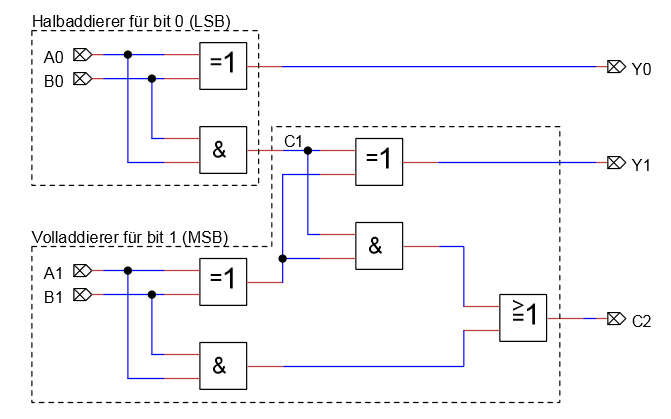
\includegraphics[scale=0.5]{./img/schaltung/Volladdierer.PNG}
    \end{center}
    \end{figure}
\end{frame}
\begin{frame}
    \frametitle{Funktionsweise}
    \framesubtitle{}
     \begin{columns}[c]
         \column{0.4\textwidth}
            \begin{block}{}
                \begin{itemize}
                    \item Die ersten Bits werden addiert
                \end{itemize}
            \end{block}
         \column{0.6\textwidth}
            \begin{figure}[H]
            \begin{center}
                    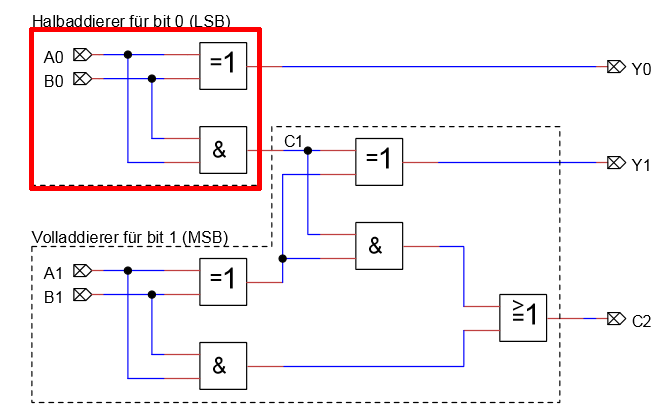
\includegraphics[scale=0.4]{./img/schaltung/Volladdierer_fun_1.png}
            \end{center}
            \end{figure}
     \end{columns}
\end{frame}
\begin{frame}
    \frametitle{Funktionsweise}
    \framesubtitle{}
     \begin{columns}[c]
         \column{0.4\textwidth}
            \begin{block}{}
                \begin{itemize}
                    \item Die ersten Bits werden addiert
                    \item Die zweiten Bits werden addiert
                \end{itemize}
            \end{block}
         \column{0.6\textwidth}
            \begin{figure}[H]
            \begin{center}
                    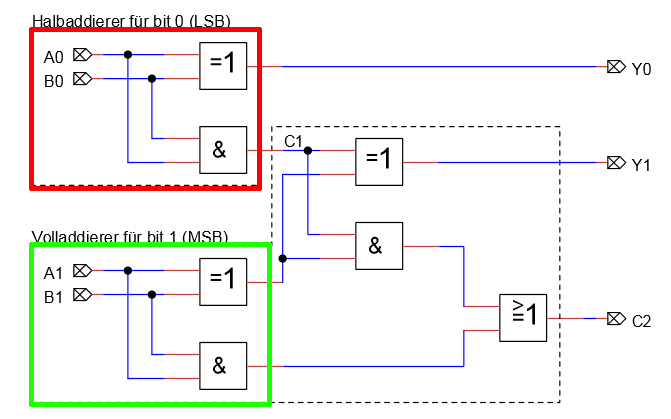
\includegraphics[scale=0.4]{./img/schaltung/Volladdierer_fun_2.png}
            \end{center}
            \end{figure}
     \end{columns}
\end{frame}
\begin{frame}
    \frametitle{Funktionsweise}
    \framesubtitle{}
     \begin{columns}[c]
         \column{0.4\textwidth}
            \begin{block}{}
                \begin{itemize}
                    \item Die ersten Bits werden addiert
                    \item Die zweiten Bits werden addiert
                    \item Das Carry der ersten Bits wird mit der Stelle der
                    zweiten addiert
                \end{itemize}
            \end{block}
         \column{0.6\textwidth}
            \begin{figure}[H]
            \begin{center}
                    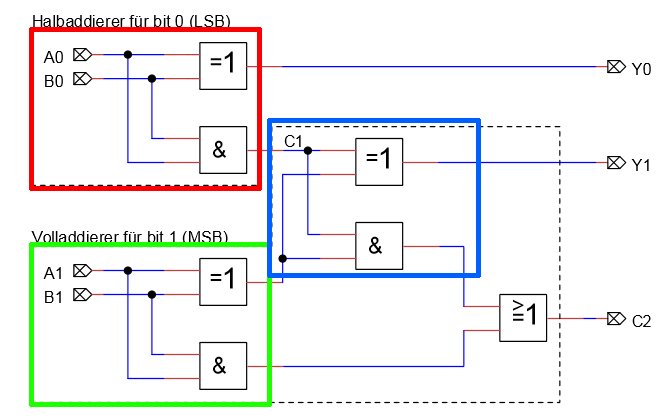
\includegraphics[scale=0.4]{./img/schaltung/Volladdierer_fun_3.png}
            \end{center}
            \end{figure}
     \end{columns}
\end{frame}
\begin{frame}
    \frametitle{Funktionsweise}
    \framesubtitle{}
     \begin{columns}[c]
         \column{0.4\textwidth}
            \begin{block}{}
                \begin{itemize}
                    \item Die ersten Bits werden addiert
                    \item Die zweiten Bits werden addiert
                    \item Das Carry der ersten Bits wird mit der Stelle der
                    zweiten addiert
                    \item ensteht bei den letzten beiden Schritten ein Übertrag
                    auf dem zweiten Bit wird dieser auf die dritte Stelle
                    geschoben
                \end{itemize}
            \end{block}
         \column{0.6\textwidth}
            \begin{figure}[H]
            \begin{center}
                    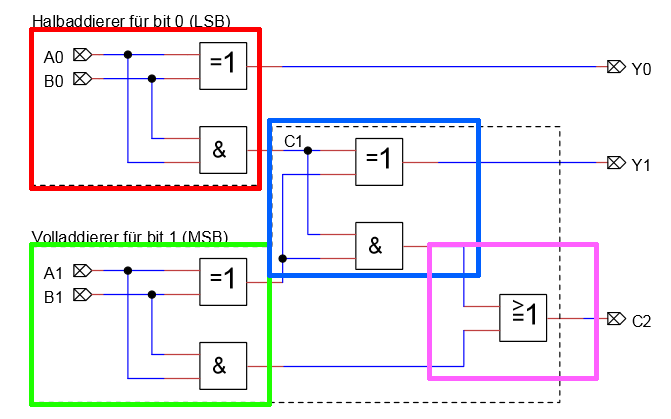
\includegraphics[scale=0.4]{./img/schaltung/Volladdierer_fun_4.png}
            \end{center}
            \end{figure}
     \end{columns}
\end{frame}
\begin{frame}
    \frametitle{}
    \framesubtitle{}
    \begin{center}
        \boxed{
            \begin{tabular}{|c|c||c||c|c||c|c|c||c|}
                A0 & B0 & C1 & A1 & B1 & Y0 & Y1 & C2 & =\\
                \hline
                0 & 0 & 0 & 0 & 0 & 0 & 0 & 0 & 0\\
                0 & 1 & 0 & 0 & 0 & 0 & 1 & 0 & 1\\
                1 & 0 & 0 & 0 & 0 & 0 & 1 & 0 & 1\\
                1 & 1 & 1 & 0 & 0 & 0 & 1 & 0 & 2\\
                \hline
                0 & 0 & 0 & 0 & 1 & 0 & 1 & 0 & 2\\
                0 & 1 & 0 & 0 & 1 & 1 & 1 & 0 & 3\\
                1 & 0 & 0 & 0 & 1 & 1 & 1 & 0 & 3\\
                1 & 1 & 1 & 0 & 1 & 0 & 0 & 1 & 4\\
                \hline
                0 & 0 & 0 & 1 & 0 & 0 & 1 & 0 & 2\\
                0 & 1 & 0 & 1 & 0 & 1 & 1 & 0 & 3\\
                1 & 0 & 0 & 1 & 0 & 1 & 1 & 0 & 3\\
                1 & 1 & 1 & 1 & 0 & 0 & 0 & 1 & 4\\
                \hline
                0 & 0 & 0 & 1 & 1 & 0 & 0 & 1 & 4\\
                0 & 1 & 0 & 1 & 1 & 1 & 0 & 1 & 5\\
                1 & 0 & 0 & 1 & 1 & 1 & 0 & 1 & 5\\
                1 & 1 & 1 & 1 & 1 & 0 & 1 & 1 & 6\\
                \hline
            \end{tabular}
            }
    \end{center}
\end{frame}
\begin{frame}
    \frametitle{Bemerkungen}
    \framesubtitle{}
    \begin{block}{}
        \begin{itemize}
            \item Volladdierer nimmt zwei 2-Bit Zahlen (dezimal 0-3) und gibt
            3-bit Zahl zurück (dezimal 0-6)
            \item $C_2$ OR kann durch XOR ersetzt werden, da niemals beide
            Eingänge gleichzeitig angesteuert werden
            \item Addition von n-bit Zahlen: n-tes Bit ist immer eine 1, d.h
            es entsteht immer ein Carry $\rightarrow$ $n+1$-bit Zahl
        \end{itemize}
    \end{block}

    
\end{frame}
% subsection Volladdierer (end)
